\documentclass[12pt]{beamer}
\usepackage[utf8x]{inputenc}
\usepackage{ucs}
\usepackage{amsmath}
\usepackage{amsfonts}
\usepackage{amssymb}
\usepackage{graphicx}
\mode<presentation>{}
\setbeamertemplate{footline}[frame number]{}
\setbeamertemplate{navigation symbols}{}

\AtBeginSection[]
  {
    \ifnum \value{framenumber}>0
      \begin{frame}<beamer>
      \frametitle{Outline}
      \tableofcontents[currentsection]
      \end{frame}
    \else
    \fi
  }

\author{Mikhail Shugay, PhD}
\title{Immune repertoire forensics}
\subtitle{A RepSeq data analysis tutorial}
\institute[Skoltech]{\texttt {Skoltech, MA03172 course [Term 2, 2017-2018]}}
\date{December 5, 2017}

\begin{document}

\maketitle

\section{Introduction}
\begin{frame}{T-cell receptor}
\begin{columns}
\column{0.55\textwidth}
\textbf{T-cell:APC contact}\\~\

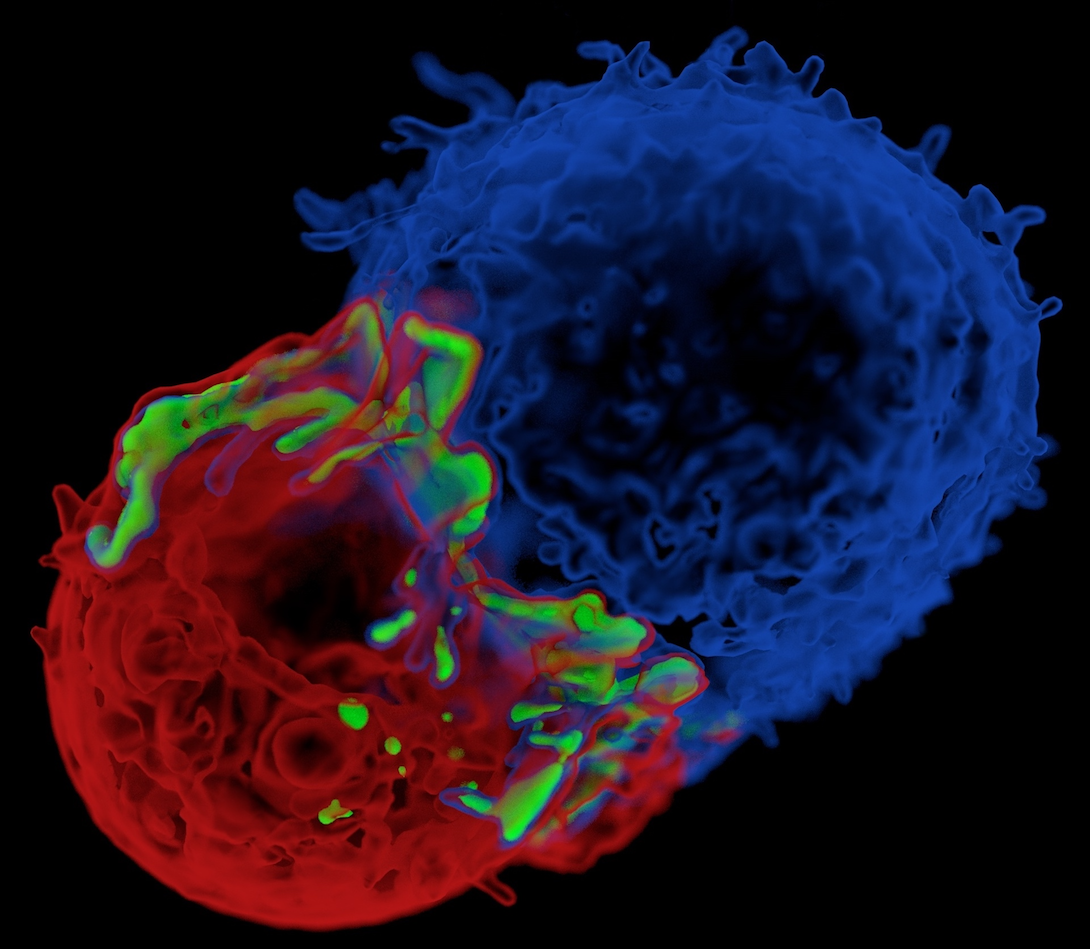
\includegraphics[scale=0.13]{p1}\\~\

From James and Vale, Nature 2012, https://valelab.ucsf.edu/images/
\pause
\column{0.45\textwidth}
\textbf{TCR:pMHC structure}\\~\

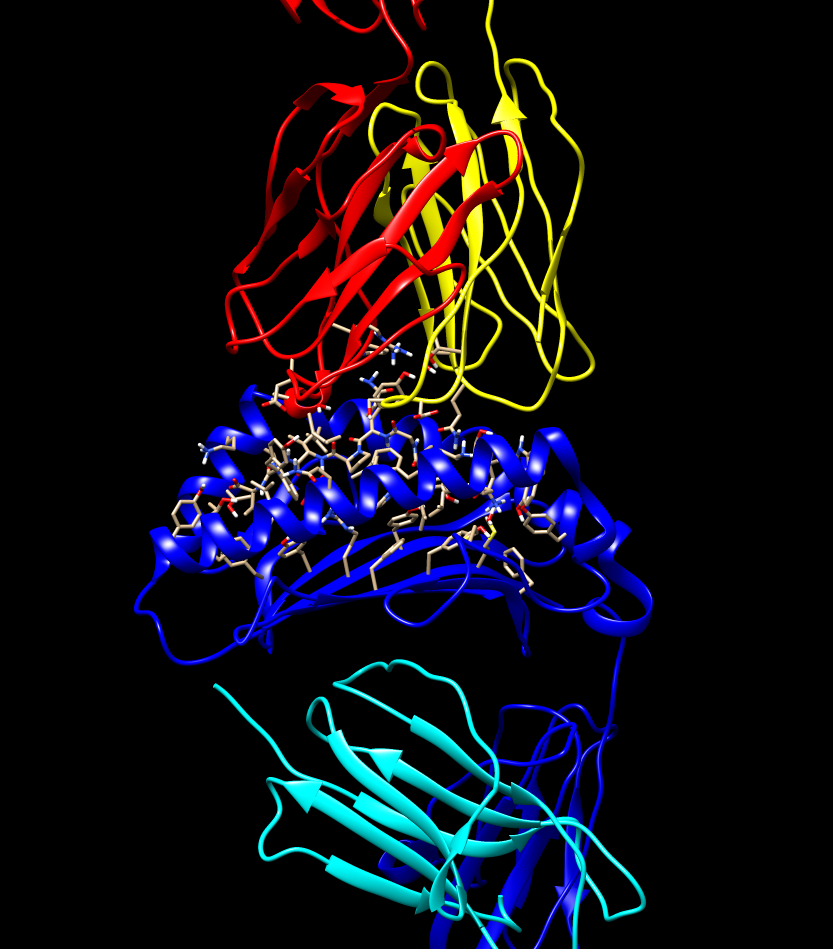
\includegraphics[scale=0.13]{p2}\\~\

PDB:1ao7, rendered using UCSF chimera, colored by chain

\end{columns}
\end{frame}

\begin{frame}{VDJ rearrangement}
An example schema for TCR$\beta$ locus
\begin{center}
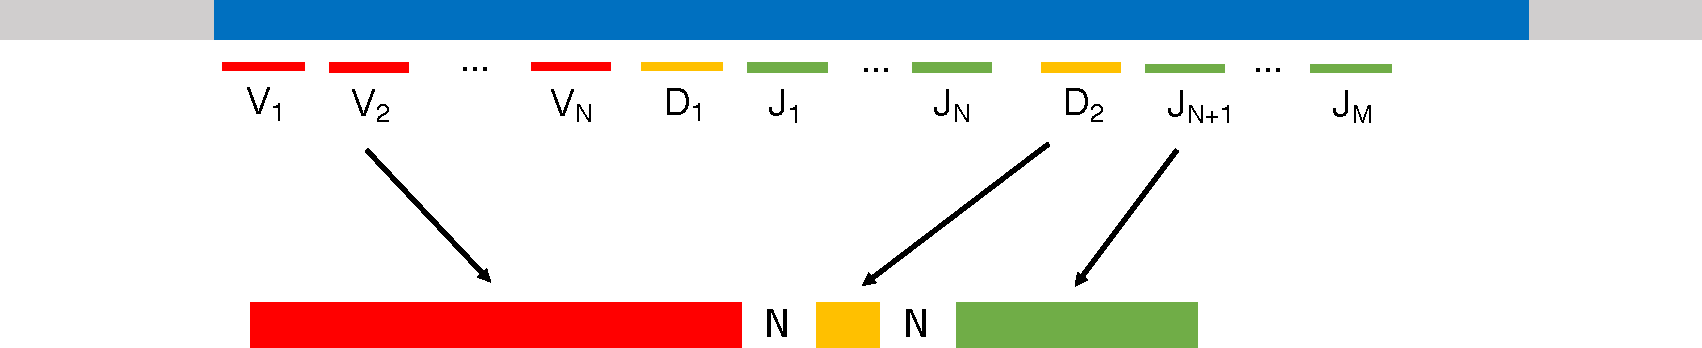
\includegraphics[width=\textwidth]{p3}
\end{center}
Variable, Diversity and Joining are chosen at random, V-D and D-J junctions are filled with non-template N bases. \\~\

\pause
VDJ rearrangement mechanism can be efficiently recaptured with a probabilistic model [\texttt{Murugan et al. PNAS 2012}]
\begin{equation*}
\begin{split}
P\left(\sigma\right) &= P(V)P(D,J) \\
 &\times P(\#del_V|V)P(\#del_J|J)P(\#del_{D5},\#del_{D3}|D) \\
 &\times P(\#ins_{VD})P(\#ins_{DJ})\prod_{i \in ins_{VD}} P(b_i|b_{i-1})\prod_{i \in ins_{DJ}} P(b_i|b_{i+1})
\end{split}
\end{equation*}
\end{frame}

\begin{frame}{TCR regions}
A TCR chains consists of the following regions:
\begin{center}
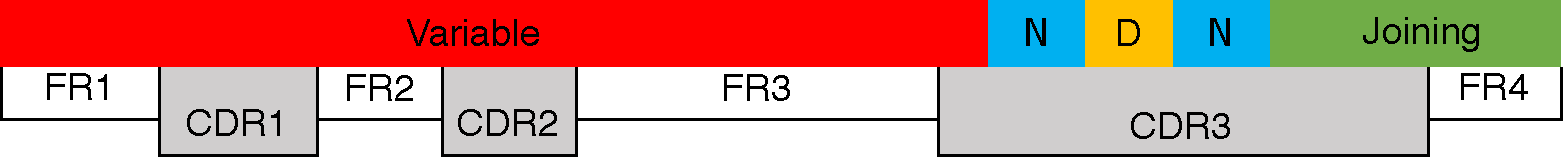
\includegraphics[width=\textwidth]{p4}
\end{center}
In total there are four framework (FRs) and three complementarity determining regions/loops (CDRs). \\~\

\pause
The likely functions of these regions are:
\begin{itemize}
\item FR regions maintain TCR secondary structure and (possibly) play role in MHC binding
\item CDR1,2 are germline encoded and play role in antigen recognition, as well as (possibly) MHC binding
\item CDR3 plays a major role in antigen recognition and is extremely variable
\end{itemize}
\end{frame}

\begin{frame}{TCR repertoire sequencing}
\begin{center}
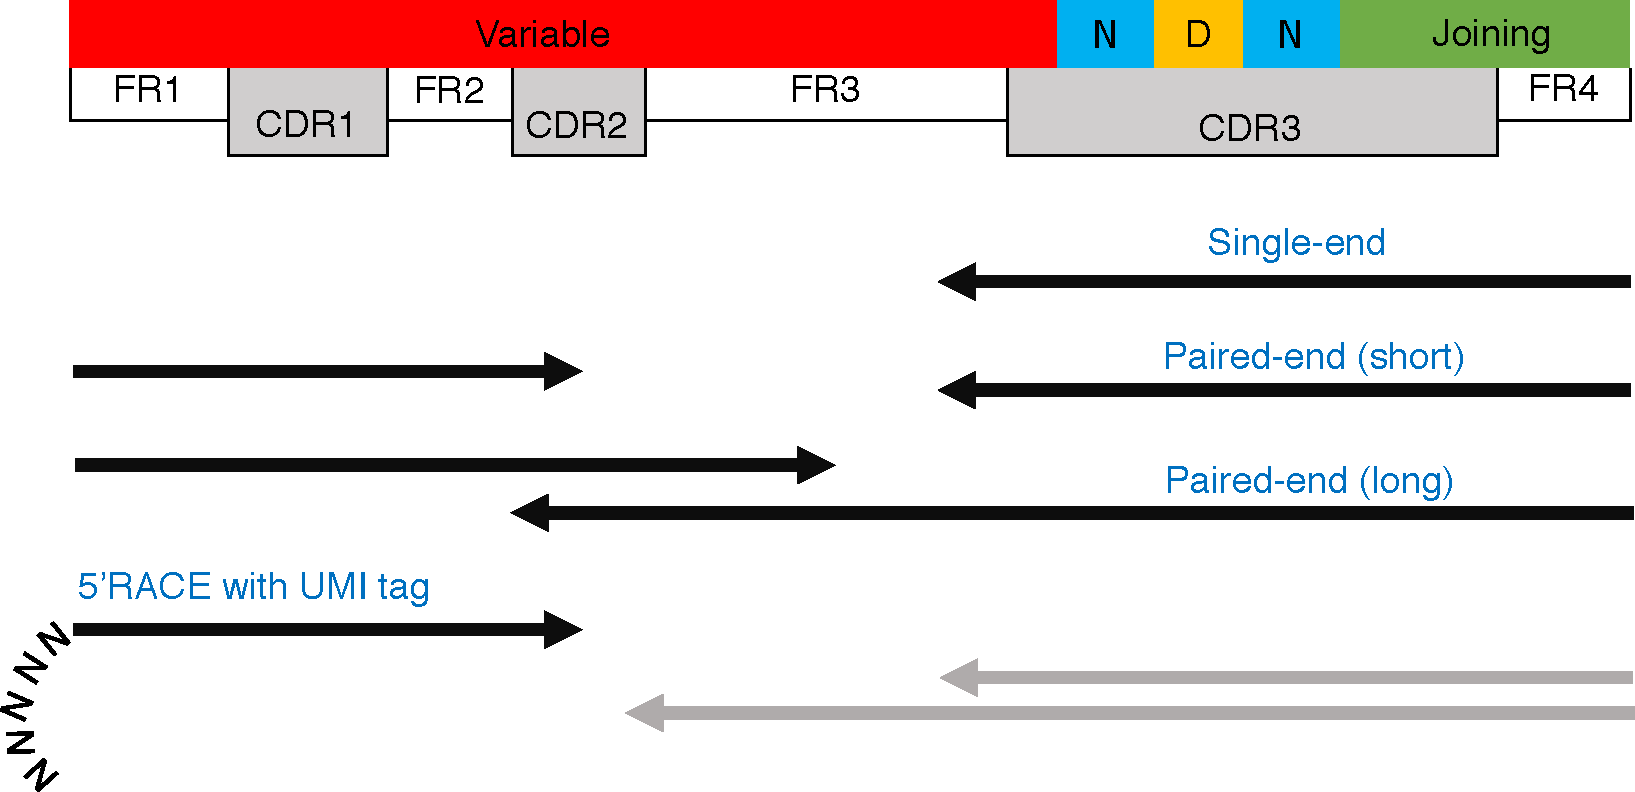
\includegraphics[width=\textwidth]{p5}
\end{center}
\end{frame}

\begin{frame}{An example of a RepSeq dataset}
After all pre-processing steps:
\begin{itemize}
\item Read grooming (filtering, etc)
\item UMI-based assembly (for molecular barcoded data)
\item V-D-J mapping and clonotype assembly\\~\
\end{itemize}

\pause
We finally get clonotype frequency tables that look like
\begin{center}
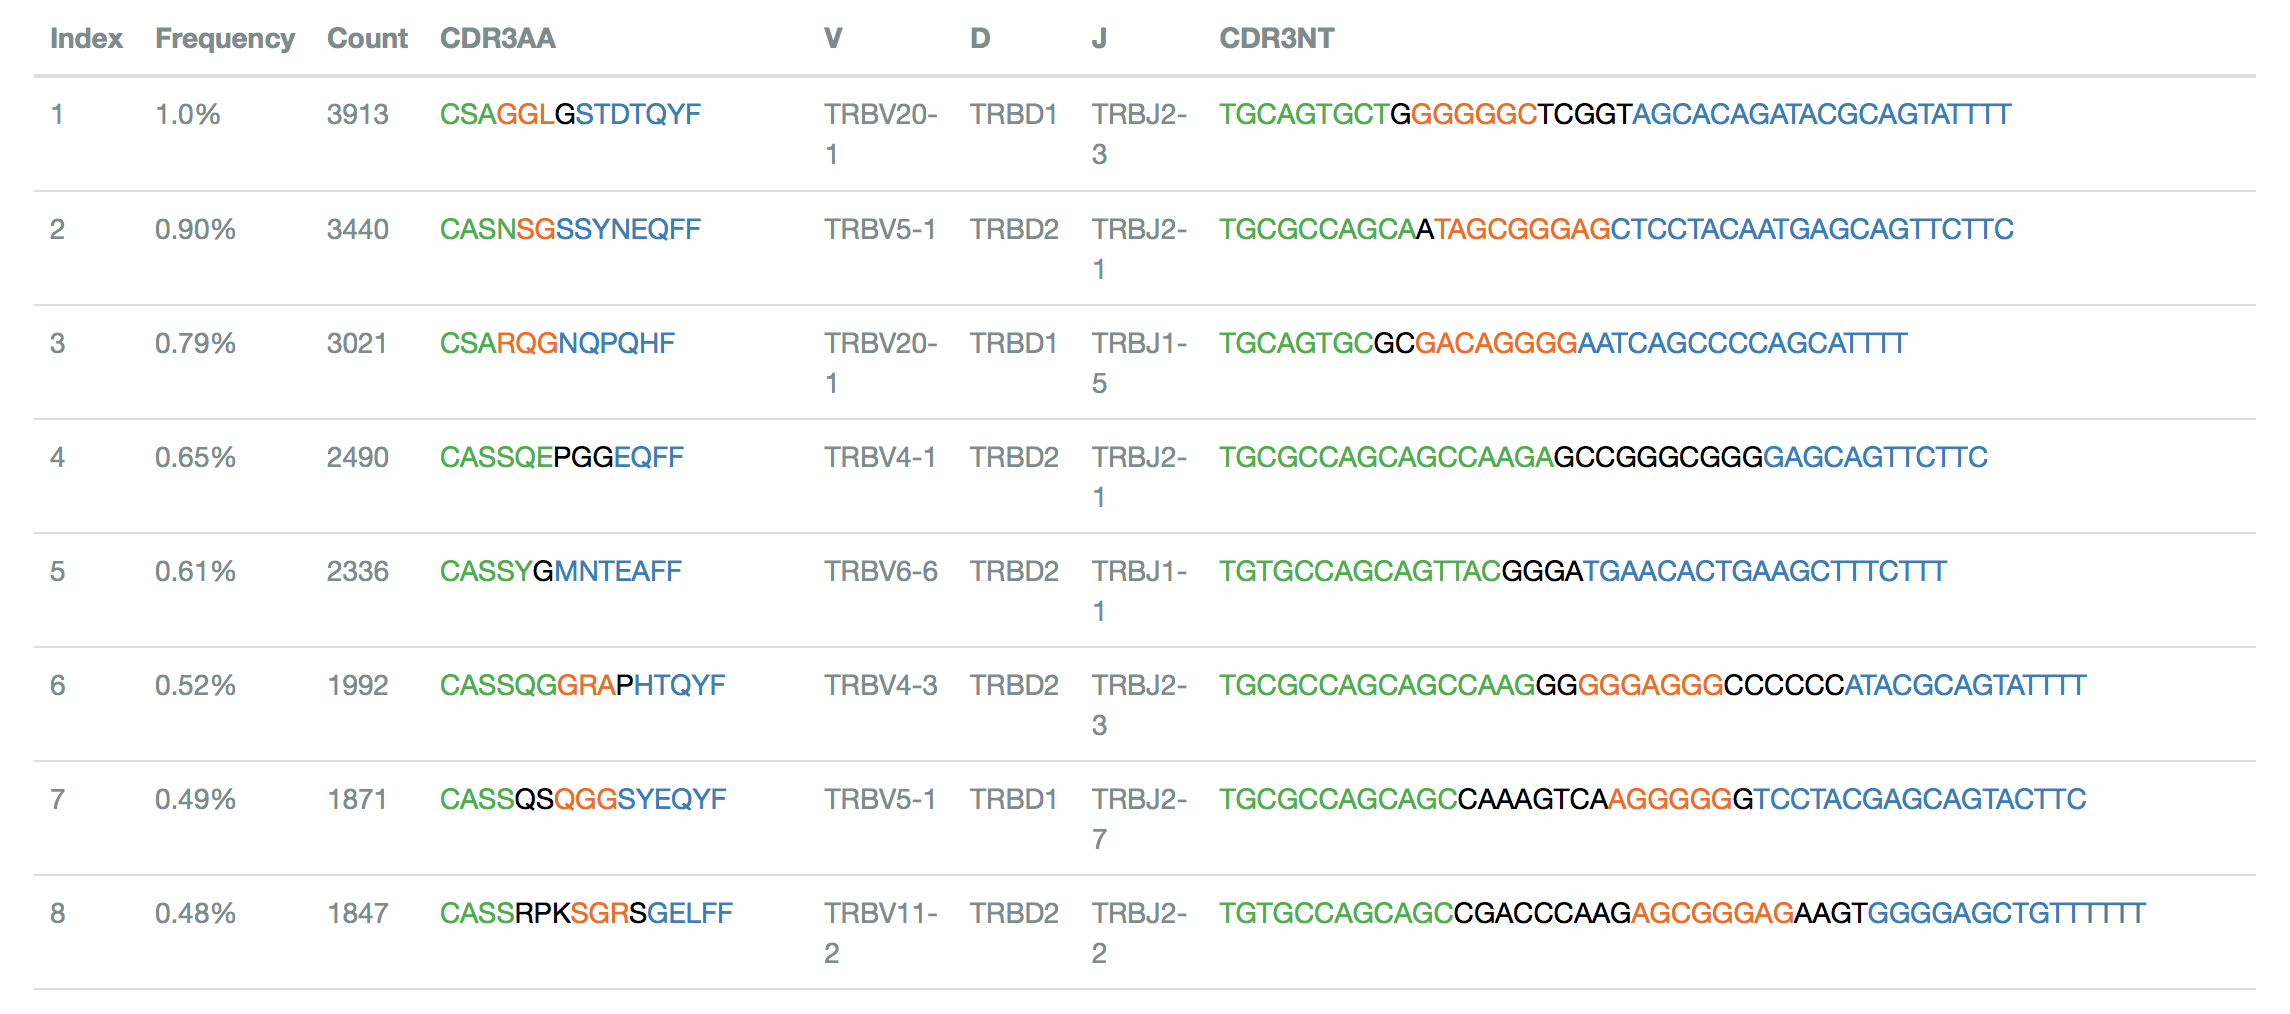
\includegraphics[width=\textwidth]{p6}
\end{center}
\end{frame}

\section{Basic RepSeq analysis methods}

\begin{frame}{Diversity analysis}
Inspired by species richness/diversity analysis in ecology. 

Useful to tell naive T-cell samples from antigen-experienced T-cells containing expanded clones.

\begin{center}
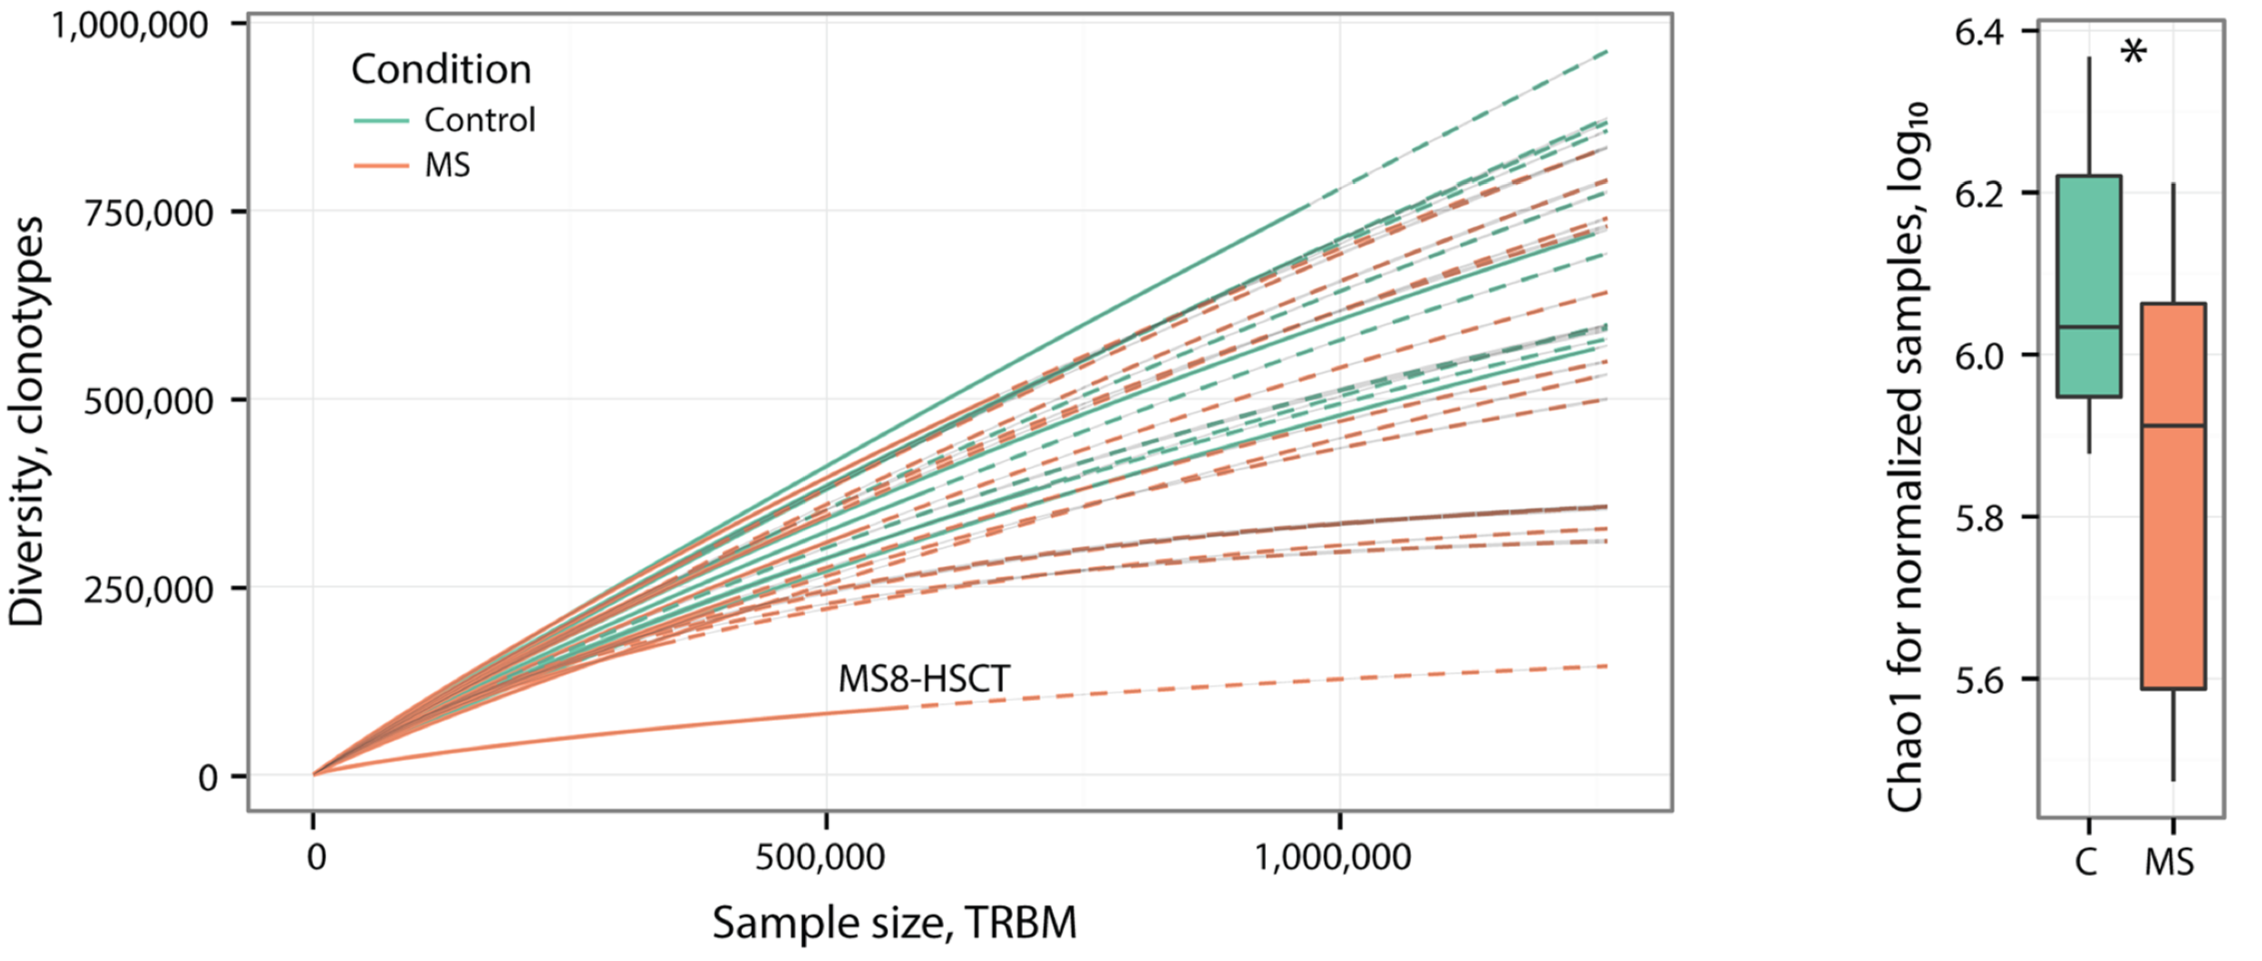
\includegraphics[scale=0.25]{p10}
\end{center}
\tiny{Shugay et al. PLoS Comp Biol 2015}
\end{frame}

\begin{frame}{Variable segment usage}
Similar to conventional gene expression analysis: segment profile can be useful for distinguishing different subsets of T-cells.
\begin{center}
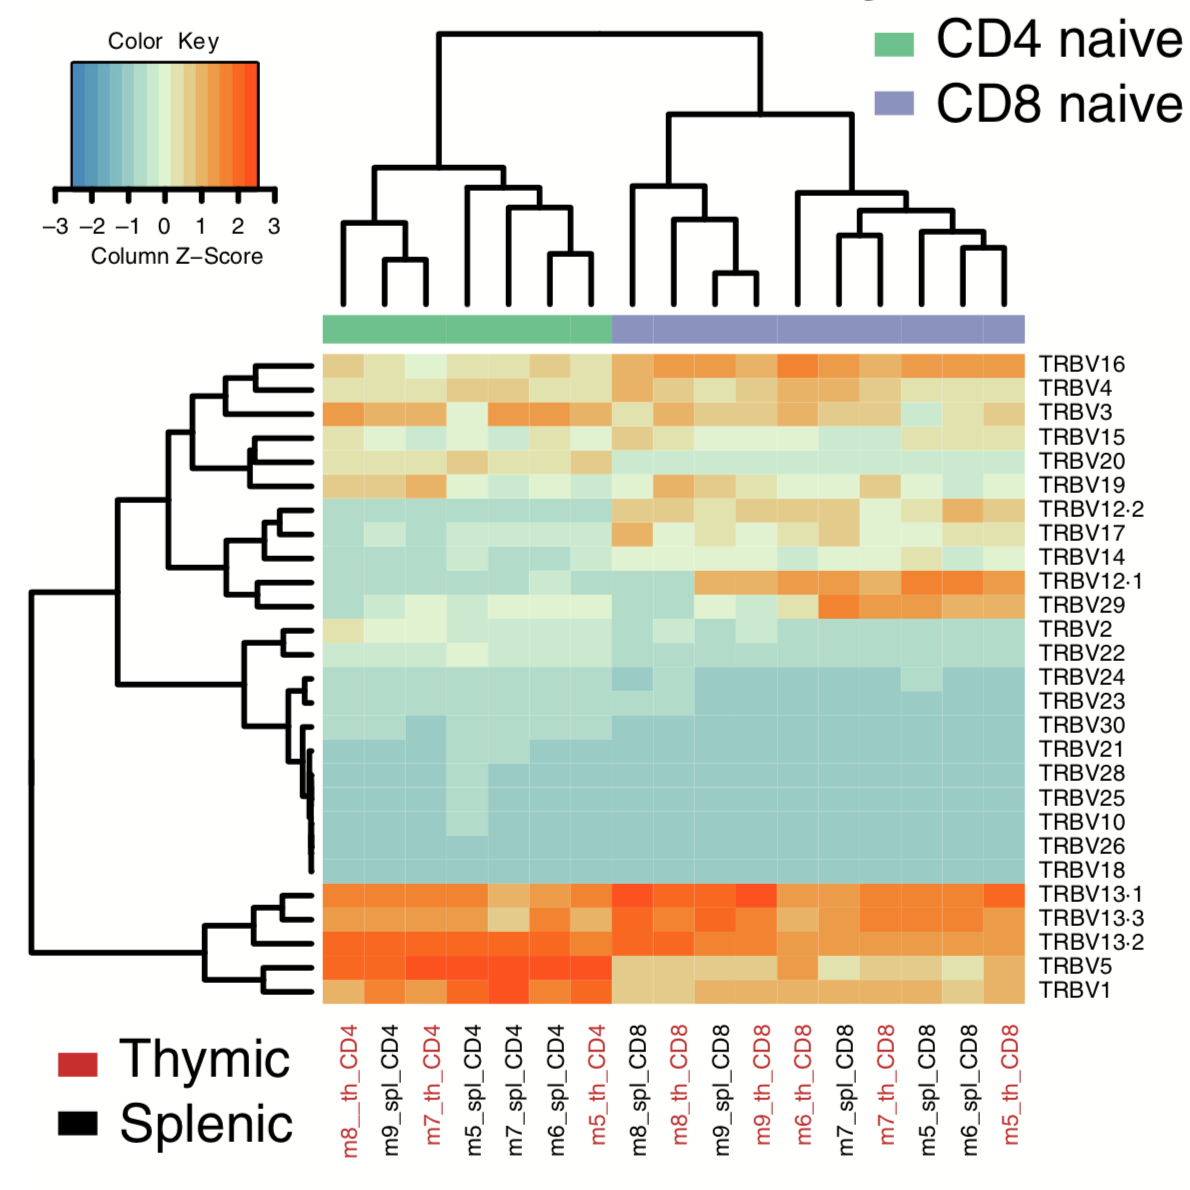
\includegraphics[scale=0.3]{p11}
\end{center}
\tiny{Izraelson et al. Immunology 2017}
\end{frame}

\begin{frame}{Clonotype sharing}
The overlap/co-incidence of hypervariable CDR3 region sequences in different samples. Useful for determining sample origin and comparative analysis of immune repertoires in general.
\begin{center}
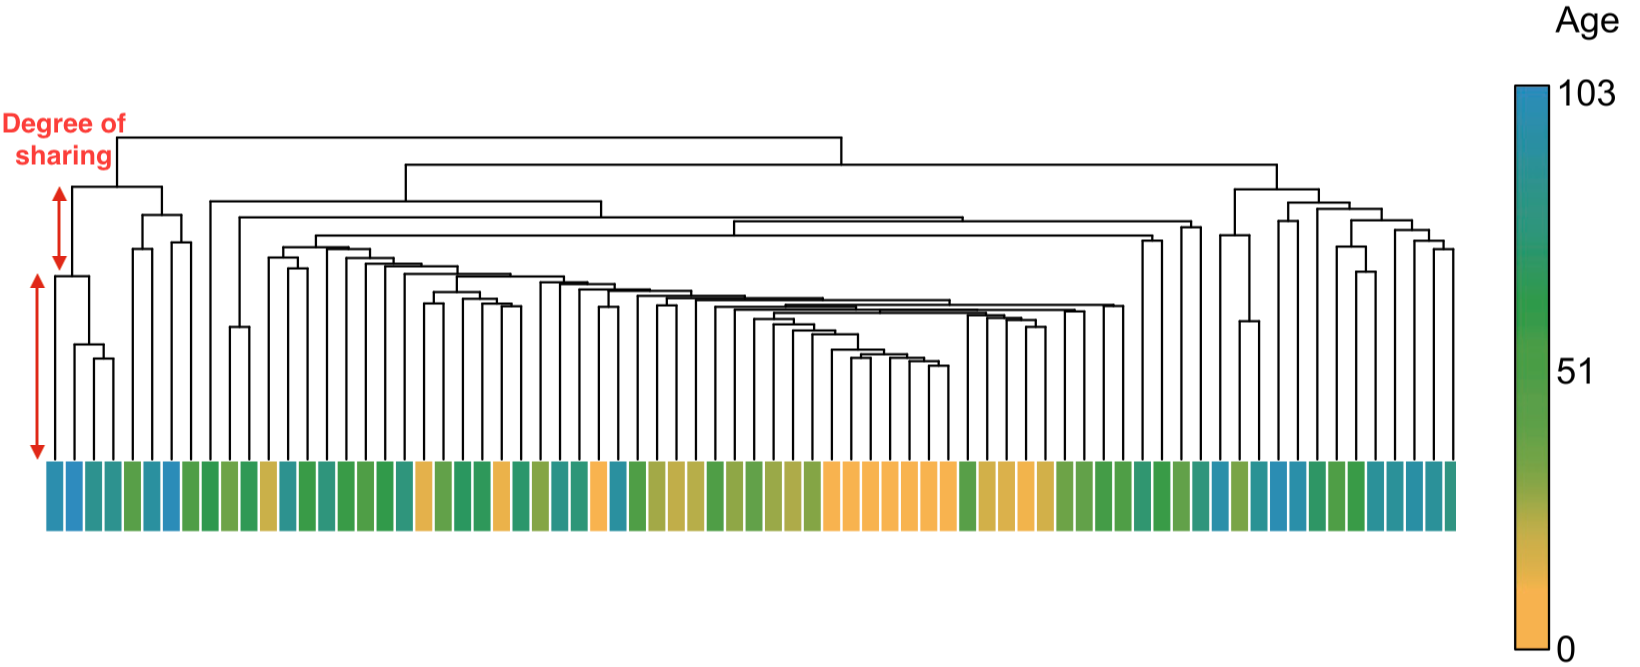
\includegraphics[scale=0.35]{p12}
\end{center}
\tiny{Britanova et al. J Immunol 2016}
\end{frame}

\begin{frame}{TCR sequence annotation}
Using a curated database of TCRs with known antigen specificity (VDJdb, \url{vdjdb.cdr3.net}). Directly searching for specific TCRs/determining the specificity profile of a repertoire.
\begin{center}
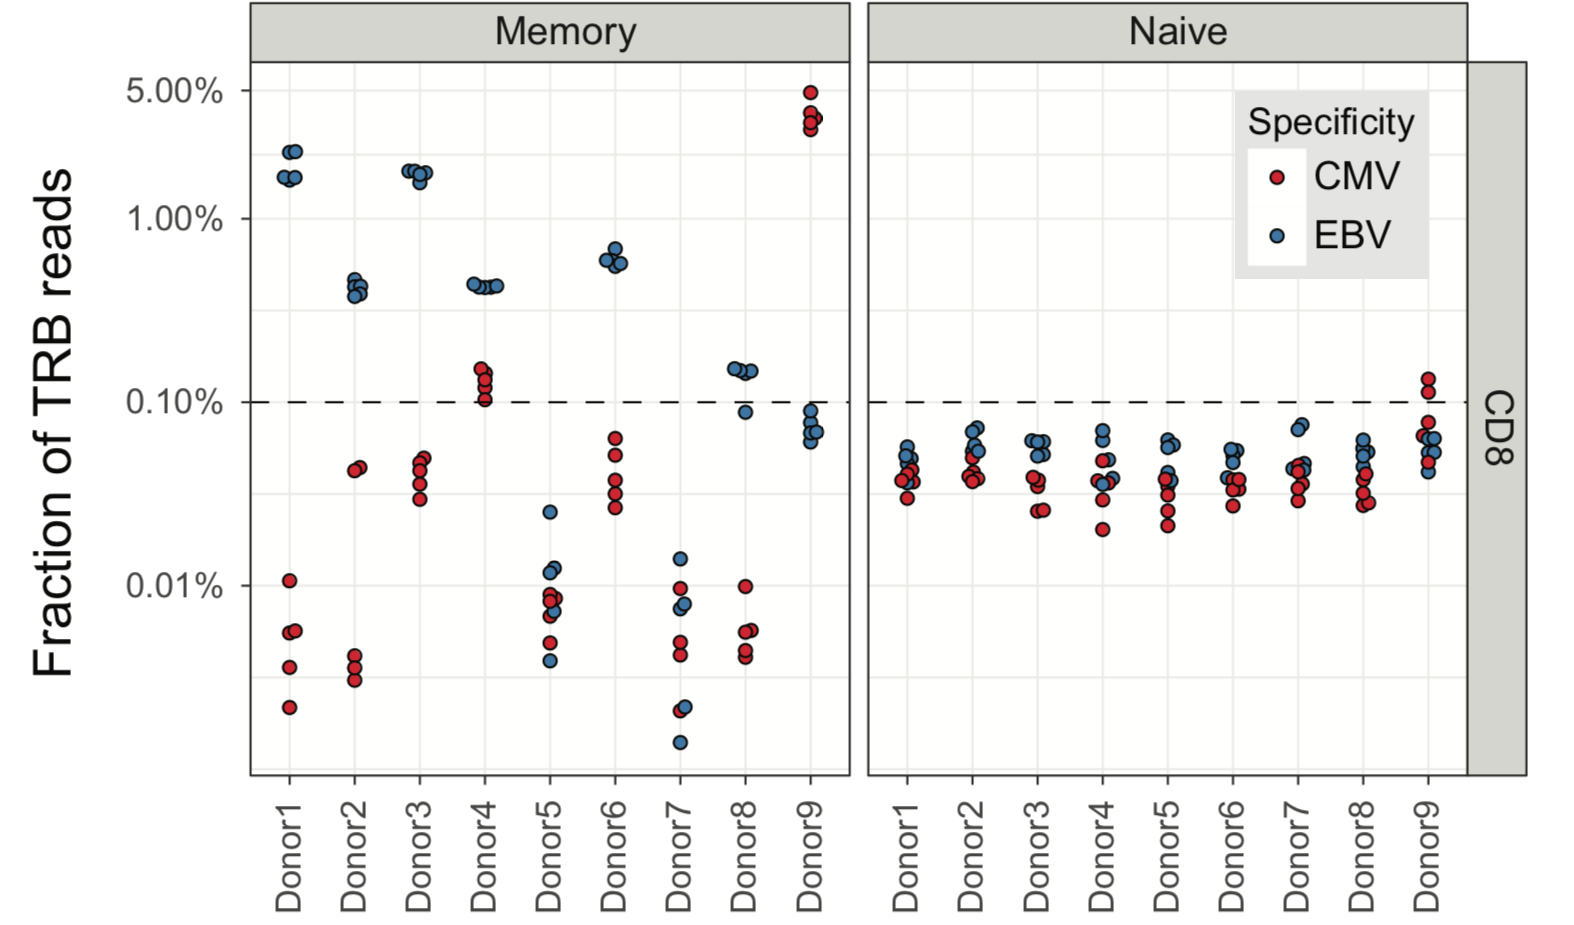
\includegraphics[scale=0.35]{p13}
\end{center}
\tiny{Shugay et al. NAR 2017}
\end{frame}

\section{Getting started}

\begin{frame}{Downloading data}
Navigate to \fbox{\url{github.com/antigenomics/repseq-forensics-tutorial}} and download the data + code bundle as zip
\begin{center}
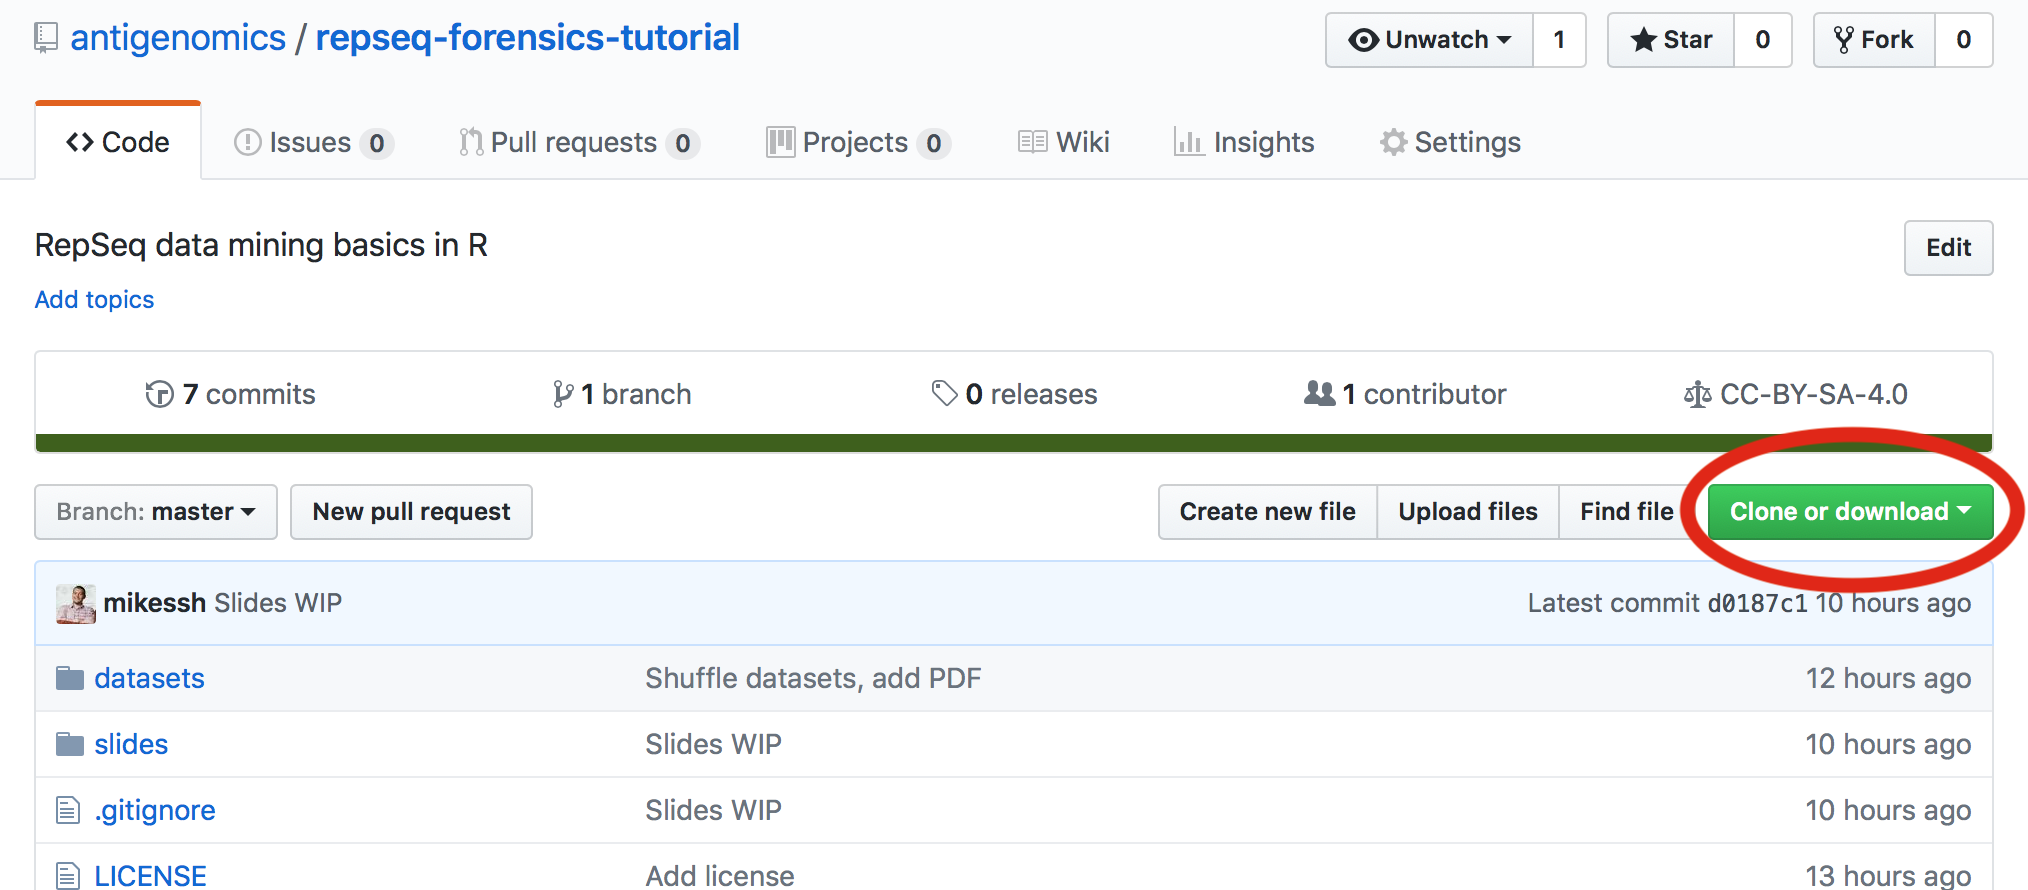
\includegraphics[width=\textwidth]{p7}
\end{center}
\end{frame}

\begin{frame}{Dataset layout}
Datasets were generated as shown in the figure below
\begin{center}
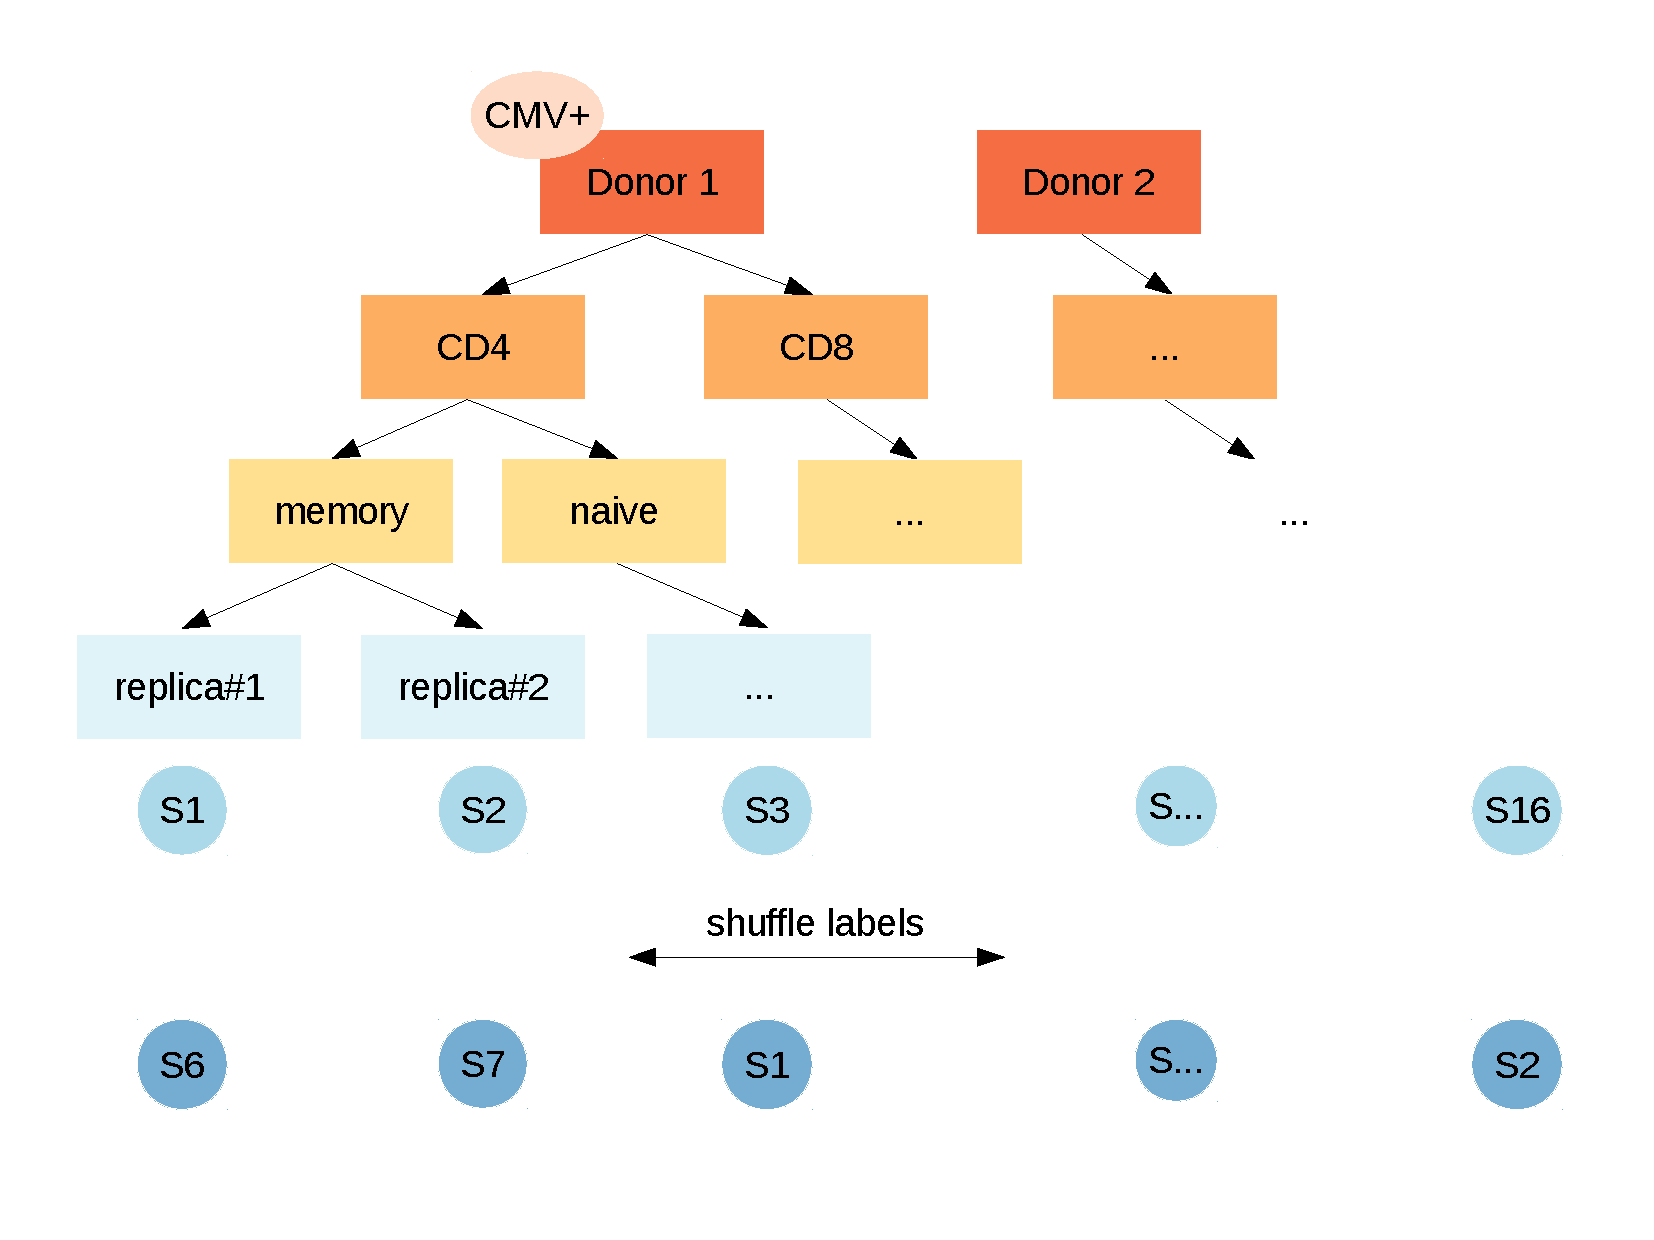
\includegraphics[width=\textwidth]{p14}
\end{center}
\end{frame}

\begin{frame}{Executing R code}
Open the \texttt{tutorial.Rmd} in RStudio, it can be found in the root folder of the bundle.
\begin{center}
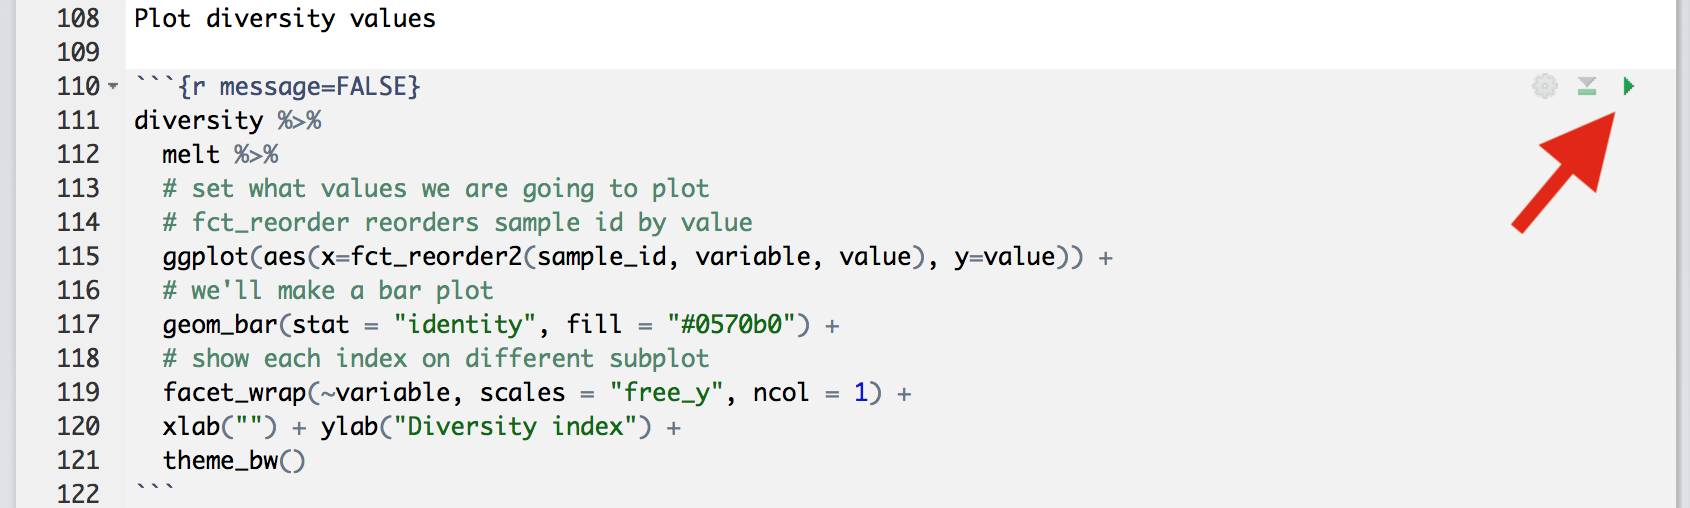
\includegraphics[width=\textwidth]{p8}
\end{center}
\end{frame}

\begin{frame}{Executing R code}
\begin{center}
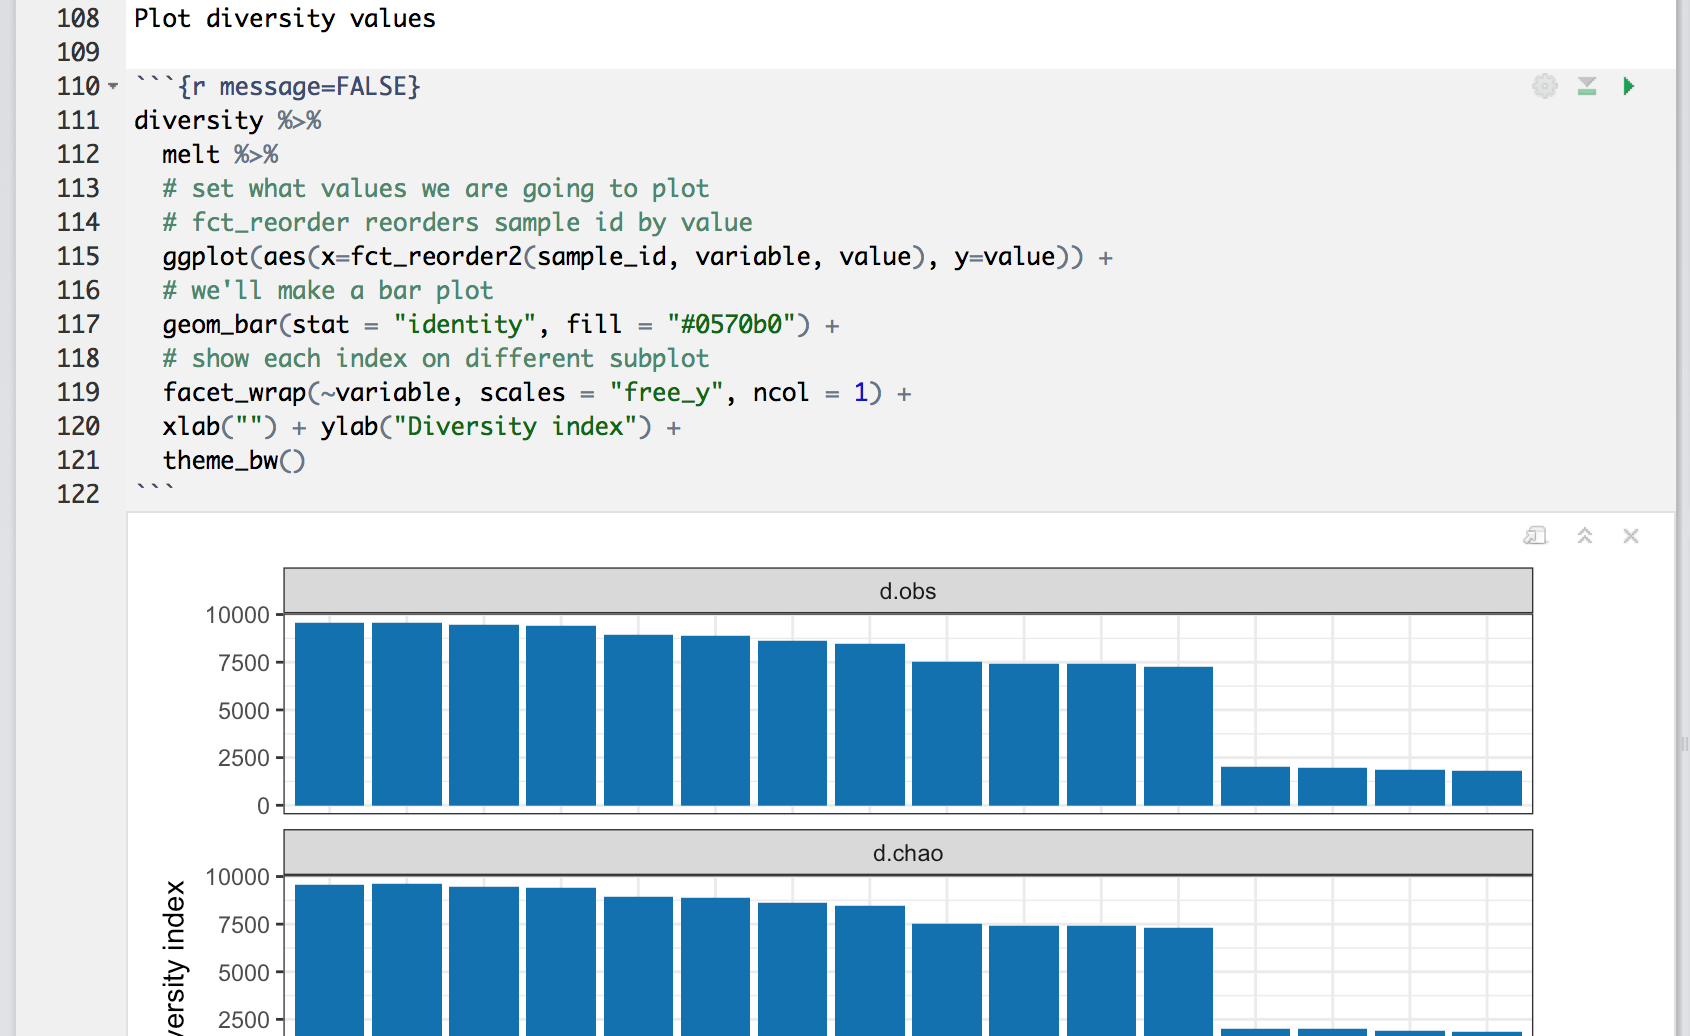
\includegraphics[width=\textwidth]{p9}
\end{center}
\end{frame}

\section{Interactive part}

\begin{frame}{Interactive part}
\begin{center}
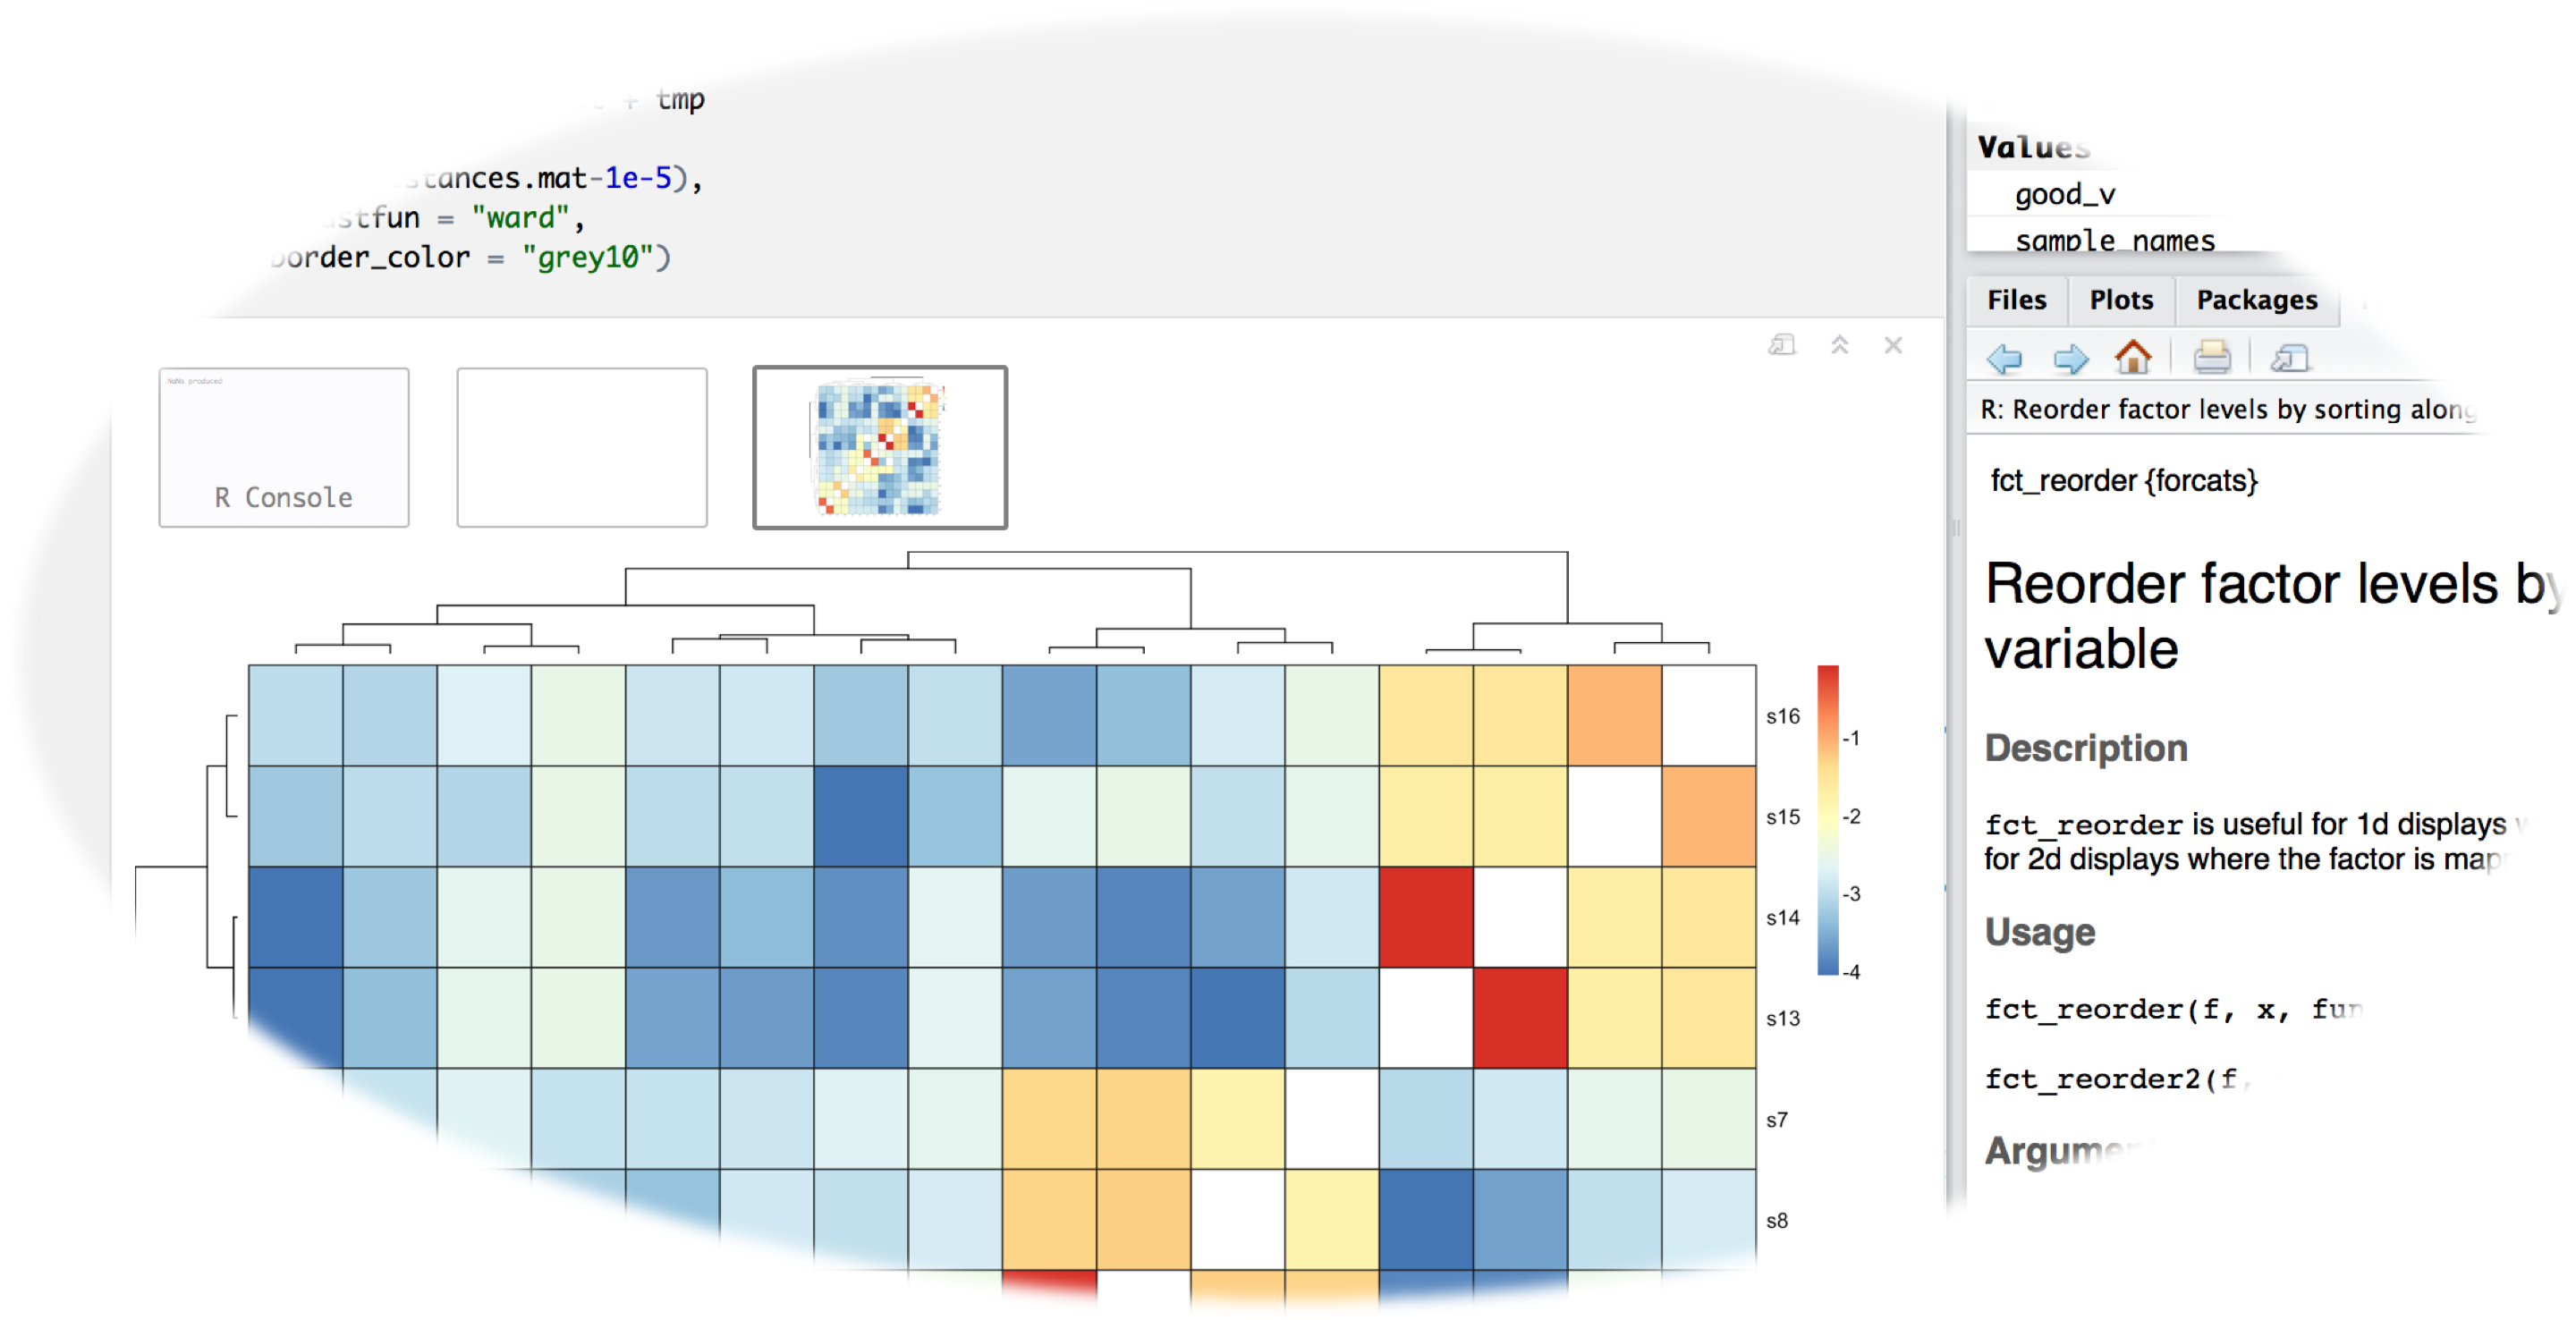
\includegraphics[width=\textwidth]{../splash}
\end{center}
\end{frame}

\section{The assignment}

\begin{frame}{The assignment}
Using the analysis results we've obtained we need to assign feature labels to each sample. Namely, you need to fill the table with the following structure:
\begin{table}[h!]
  \begin{center}
    \begin{tabular}{c|c|c|c|c}
      \textbf{sample} & \textbf{donor} & \textbf{subset} & \textbf{phenotype} & \textbf{CMVstatus} \\
      \hline
      s1 & D1 & CD4 & memory & CMV- \\
      s2 & D2 &   & naive & CMV+ \\
      s3 & D1 & CD8 & naive & CMV- \\
      ... & ... & ... & ... & ... \\
    \end{tabular}
  \end{center}
\end{table}
\end{frame}

\begin{frame}{Details}
Table filling rules:
\begin{itemize}
\item Column names should match those on previous slide
\item Sample id should be one of $s_1..s_{16}$
\item Two distinct donor IDs should be used, naming doesn't matter
\item Subset should be either \textbf{CD4} or \textbf{CD8}
\item Phenotype should be either \textbf{memory} or \textbf{naive}
\item CMV status should be either \textbf{CMV+} or \textbf{CMV-}
\item Unknown/ambiguous fields should be left blank
\end{itemize}
\end{frame}

\begin{frame}{A hint}
While you can unambiguously assign CD4/8 and memory/naive labels, as well as point out biological replicates of the same sample, assigning donor labels is tricky.\\~\

First, it is impossible to link CD4-CD8 cells of the same donor. Same for CMV status, that is unambiguous only for CD8+ memory T-cells. Therefore I expect that you mark donors in the way they will distinguish samples/replicas coming from the same and different donors.\\~\

I.e. there is no problem if donor labels are swapped between CD4 and CD8 T-cells as far as they point to distinct donors for CD4 or CD8 T-cells coming from different donor and the same donor for replicas.
\end{frame}

\begin{frame}{Feedback}
Send me filled tables to \fbox{\_\_\_@gmail.com}:
\begin{itemize}
\item As plain text tab-delimited files
\item Mail title should start with \fbox{REPSEQ-TUTORIAL}.
\item Attachment name should be in \fbox{your-name.assignment.txt} format.
\end{itemize}
\end{frame}

\begin{frame}{Final remarks}
\begin{LARGE}
\begin{center}
Thanks for your attention!\\~\
\end{center}
\end{LARGE}


These slides and a PDF file containing compiled analysis results can be found in \texttt{slides/} and root folders of the data and code bundle.
\end{frame}

\end{document}